%% OPSEARCH submission -- Springer Nature LaTeX template (sn-jnl, Version 3.1 Dec 2024).
%% Built into a flat upload folder by scripts/build_submission.py; do not compile this file directly.
\documentclass[pdflatex,sn-basic]{sn-jnl}

\usepackage[T1]{fontenc}%
\usepackage{graphicx}%
\usepackage{amsmath,amssymb,amsfonts}%
\usepackage{xcolor}%
\usepackage{booktabs}%
\usepackage{caption}%
\usepackage{adjustbox}%
\usepackage{tikz}%
\usetikzlibrary{positioning,arrows.meta}%
\usepackage{xurl}%

\newcommand{\todo}[1]{\textcolor{red}{[\textbf{TODO:} #1]}}
\newcommand{\INR}{INR~}

%% Submission metadata to complete before upload (see submission/opsearch/README.md)
\newcommand{\RepoURL}{\url{https://github.com/MadhavGupta27/price-of-speed.git}}

% ---- begin generated/numbers.tex
% Generated by scripts/export_numbers.py -- do not edit
\newcommand{\AreaKm}{720}
\newcommand{\NDemandCells}{3,426}
\newcommand{\NOsmSites}{1,480}
\newcommand{\NCandidates}{1,133}
\newcommand{\PopWorldPop}{6.04}
\newcommand{\Detour}{1.57}
\newcommand{\DetourLo}{1.41}
\newcommand{\DetourHi}{1.81}
\newcommand{\KaggleOffsetPct}{98.4}
\newcommand{\CurrentStores}{440}
\newcommand{\BaseV}{15}
\newcommand{\BaseT}{15}
\newcommand{\StoresTTen}{320}
\newcommand{\CostPerOrderTen}{43.4}
\newcommand{\ServedTenPct}{86.7}
\newcommand{\RidersTen}{6,902}
\newcommand{\StoresTFifteen}{240}
\newcommand{\CostPerOrderFifteen}{43.2}
\newcommand{\ServedFifteenPct}{98.3}
\newcommand{\RidersFifteen}{9,275}
\newcommand{\StoresTTwenty}{239}
\newcommand{\CostPerOrderTwenty}{43.9}
\newcommand{\ServedTwentyPct}{99.9}
\newcommand{\RidersTwenty}{9,700}
\newcommand{\StoresTThirty}{238}
\newcommand{\CostPerOrderThirty}{43.9}
\newcommand{\ServedThirtyPct}{100.0}
\newcommand{\RidersThirty}{9,733}
\newcommand{\UnreachTenPct}{13.3}
\newcommand{\CostPerOrderVTwelve}{49.3}
\newcommand{\CostPerOrderVTwenty}{36.3}
\newcommand{\SpeedCapPremiumPct}{19}
\newcommand{\StoreRange}{202--390}
\newcommand{\PertTenP}{99.7}
\newcommand{\PertTenSpeed}{12.1}
\newcommand{\AssignStressTenOnTime}{64}
\newcommand{\AssignStressSpeed}{20}
\newcommand{\AssignStressRide}{1.3}
\newcommand{\TransLP}{5.80}
\newcommand{\TransVAM}{5.85}
\newcommand{\TransNW}{13.29}
\newcommand{\TransNearest}{5.60}
\newcommand{\TransVAMGapPct}{0.9}
\newcommand{\TransNWRatio}{2.3}
\newcommand{\TransCapPremiumPct}{3.5}
\newcommand{\GridTenStores}{462}
\newcommand{\GridTenServedPct}{100.0}
\newcommand{\GridTenCost}{45.9}
\newcommand{\GridFifteenStores}{287}
\newcommand{\GridFifteenCost}{42.4}
\newcommand{\GridStorePremiumPct}{61}
\newcommand{\GridCostPremiumPct}{8.4}
\newcommand{\GridPricePerMinute}{0.71}
\newcommand{\GridCandidates}{860}
\newcommand{\TornadoTop}{rider cost}
\newcommand{\TornadoSecond}{rider utilisation}
\newcommand{\TornadoTopSpan}{13.4}
\newcommand{\TornadoSecondSpan}{11.0}
\newcommand{\FragTenOne}{74.6}
\newcommand{\FragFifteenOne}{98.3}
\newcommand{\FragTenMax}{86.7}
\newcommand{\FragFifteenHundred}{98.1}
\newcommand{\MixedStores}{318}
\newcommand{\MixedTenShare}{86.7}
\newcommand{\MixedServed}{98.3}
\newcommand{\MixedCost}{45.0}
\newcommand{\MixedPremiumPct}{4.2}
\newcommand{\MixedExtraStores}{78}
\newcommand{\NMilps}{29}
\newcommand{\NMilpsOptimal}{27}
\newcommand{\NMilpsLimit}{2}
\newcommand{\MaxSolveS}{154}
% ---- end generated/numbers.tex

% ---- begin generated/biblio_numbers.tex
% Generated by scripts/build_lit_assets.py -- do not edit
\newcommand{\BibIdentified}{7,576}
\newcommand{\BibAfterMethod}{715}
\newcommand{\BibScreened}{216}
\newcommand{\BibIncluded}{168}
\newcommand{\BibExcluded}{48}
\newcommand{\BibExclScope}{37}
\newcommand{\BibExclNoOR}{10}
\newcommand{\BibExclIntro}{1}
\newcommand{\BibSearchDate}{2026-10-06}
\newcommand{\BibGrowthPct}{31.4}
\newcommand{\BibSinceTwentyOnePct}{91}
\newcommand{\BibYearsTwentyFive}{46}
\newcommand{\BibTopJournal}{European Journal of Operational Research}
\newcommand{\BibTopJournalN}{20}
\newcommand{\BibSecondJournal}{Computers \& Operations Research}
\newcommand{\BibSecondJournalN}{14}
\newcommand{\BibDrones}{54}
\newcommand{\BibAssign}{50}
\newcommand{\BibLocation}{23}
\newcommand{\BibOnDemand}{27}
\newcommand{\BibQComm}{3}
\newcommand{\BibIndia}{0}
\newcommand{\BibWelfare}{4}
\newcommand{\BibPromise}{4}
\newcommand{\BibReviews}{9}
\newcommand{\BibMILPKw}{49}
\newcommand{\BibALNSKw}{17}
% ---- end generated/biblio_numbers.tex


\raggedbottom

\begin{document}

\title[The Price of Speed]{The Price of Speed: Optimising Dark-Store Networks and Rider Assignment under Relaxed Delivery Promises in Indian Quick Commerce}

\author*[1]{\fnm{Madhav} \sur{Gupta}}\email{madhavgupta270407@gmail.com}
\author[1]{\fnm{Aadee} \sur{Pardasani}}
\author[1]{\fnm{Aashi} \sur{Khuthia}}
\author[1]{\fnm{Jiya} \sur{Jagawat}}
\author[1]{\fnm{Prishi} \sur{Doshi}}
\author[1]{\fnm{Aarushi} \sur{Rakesh}}

\affil*[1]{\orgname{NMIMS University}, \orgaddress{\city{Mumbai}, \country{India}}}

% ---- begin src/abstract_journal.tex
\abstract{In January 2026 India's quick-commerce platforms withdrew their ``10-minute delivery'' claims after the Union Labour Ministry raised rider-safety concerns, and in August 2026 a Parliamentary Standing Committee recommended curbs on ``unrealistic speed targets'' without defining them. We combine a bibliometric review of \BibIncluded{} operations research articles on last-mile and on-demand delivery (2015--2026) with an integrated optimisation model of a Bengaluru dark-store network built entirely from public data. A coverage-constrained facility-location model opens stores and allocates demand at minimum store and rider cost while guaranteeing a promise $T$ at a safe rider speed $v$; a transportation model plans replenishment, an assignment model dispatches riders at peak, and a PERT model estimates on-time probability. At \BaseV~km/h the cost-optimal network has about \StoresTFifteen{} stores and reaches \ServedFifteenPct\% of residents for any promise of 15 minutes or more, whereas a 10-minute promise leaves \UnreachTenPct\% unreachable from available retail sites; serving everyone within 10 minutes requires \GridStorePremiumPct\% more stores and \GridCostPremiumPct\% higher cost per order. Rider speed, not the promise, drives cost: a 15 rather than 20~km/h cap raises cost per order by about \SpeedCapPremiumPct\%. We propose reachability within a safe ride radius as an operational definition of a ``realistic'' promise: promising 10 minutes only where reachable gives \MixedTenShare\% of residents 10-minute service at \MixedPremiumPct\% higher cost than a uniform 15-minute network.}
% ---- end src/abstract_journal.tex


\keywords{quick commerce, dark stores, facility location, transportation problem, assignment problem, PERT, bibliometric analysis, gig-worker safety, India}

\maketitle

% ---- begin sections/introduction
\section{Introduction}\label{sec:intro}

Quick commerce (q-commerce) promises groceries and household essentials within minutes, fulfilled from small urban warehouses called \emph{dark stores}. India has become its largest laboratory: in the April--June 2026 quarter Blinkit alone reported 2,443 dark stores and 331 million orders \citep{eternal2026q1}, and Swiggy Instamart a further 1,171 stores \citep{swiggy2026q1}. The model rests on a simple geometry: a store that serves only a 1.5--3~km radius can meet a 10-minute promise without riders travelling fast, which is how platform founders defended it \citep{palicha2022,dhindsa2021}.

That defence has been tested. After a nationwide strike by gig workers on 31 December 2025, the Union Labour Ministry intervened and in January 2026 Blinkit, Zepto, Swiggy Instamart and Zomato dropped ``10-minute delivery'' from their branding \citep{outlook2026drop}. In August 2026 the Parliamentary Standing Committee on Commerce recommended guidelines against ``unrealistic speed targets'' set by dispatch algorithms, but did not say what makes a target unrealistic \citep{outlook2026panel}. The policy debate therefore lacks a quantitative answer to a classical OR question: \emph{what does each minute of delivery promise cost, and who pays for it---the platform, through more stores, or the rider, through higher speed?}

This paper answers that question for Bengaluru, India's most contested q-commerce market, and situates it in the OR literature. We pose three research questions:

\begin{description}
  \item[RQ1] How has OR research on on-demand and last-mile delivery evolved, which methods dominate (location, assignment, routing), and where are the gaps for quick commerce and courier welfare?
  \item[RQ2] For Bengaluru, how do the number of dark stores, rider requirements and cost change as the delivery promise relaxes from 10 to 15, 20 and 30 minutes under a safety-capped rider speed?
  \item[RQ3] Which promise level and network design balance coverage, cost and rider safety, and what does this imply for defining a ``realistic'' speed target?
\end{description}

Our contributions are fourfold. First, a bibliometric map of OR research on last-mile and on-demand delivery from 2015 to 2026, which shows a fast-growing field (\BibGrowthPct\% a year) centred on vehicle routing with new delivery modes, in which only \BibQComm{} of \BibIncluded{} articles address quick commerce, none studies India and only \BibWelfare{} consider courier welfare. Second, an integrated and fully reproducible model chain---coverage-constrained facility location, transportation, assignment and PERT---built from public Indian data, together with an audit showing why widely used Kaggle delivery datasets are unsuitable for spatial modelling. Third, a ``price of speed'' curve for Bengaluru. Fourth, evidence for regulators on where a delivery promise stops being achievable through network design and starts depending on rider speed.

Section~\ref{sec:lit} reviews the literature; Section~\ref{sec:method} describes the bibliometric protocol and modelling framework; Section~\ref{sec:data} presents the case and data; Section~\ref{sec:model} formulates the models; Section~\ref{sec:results} reports results; Section~\ref{sec:discussion} discusses implications and limitations; Section~\ref{sec:conclusion} concludes.
% ---- end sections/introduction

% ---- begin sections/literature
\section{Literature review}\label{sec:lit}

\subsection{Bibliometric overview}

The search (Section~\ref{sec:method}) yielded \BibIncluded{} journal articles on OR for last-mile and on-demand delivery published between 2015 and 2026. The field is young and accelerating: output grew at \BibGrowthPct\% a year between 2015 and 2025, \BibSinceTwentyOnePct\% of the corpus appeared from 2021 onwards, and 2025 alone contributed \BibYearsTwentyFive{} articles (Figure~\ref{fig:annual}). Core OR journals dominate: the \emph{\BibTopJournal} published \BibTopJournalN{} articles and \emph{\BibSecondJournal} \BibSecondJournalN, followed by \emph{Transportation Research Procedia} and the \emph{Annals of Operations Research}.

\begin{figure}[ht]
\centering
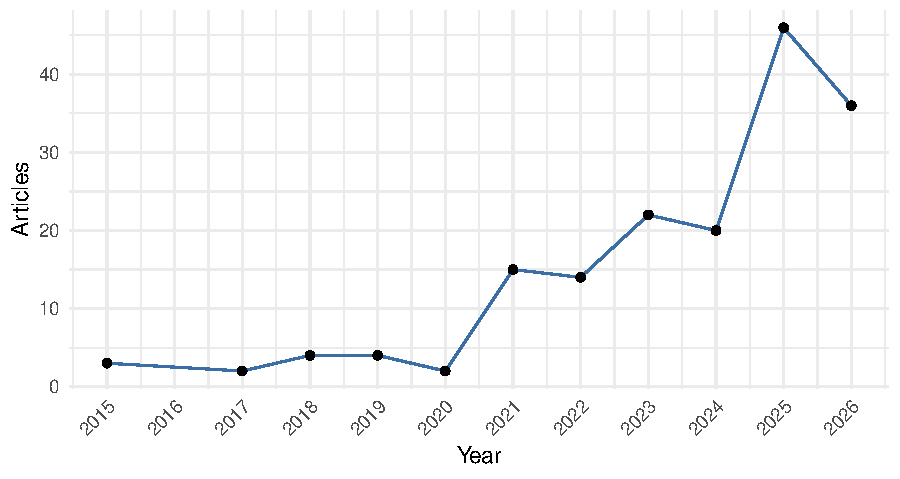
\includegraphics[width=\linewidth]{annual_production.pdf}
\caption{Annual number of included articles (2026 is a partial year).}\label{fig:annual}
\end{figure}

The most frequent keywords (Figure~\ref{fig:cooc}) are \emph{last-mile delivery} and \emph{vehicle routing}, with mixed-integer programming (\BibMILPKw{} keyword occurrences) and adaptive large neighbourhood search (\BibALNSKw) as the dominant solution technologies. Counting topics across titles, abstracts and keywords, drones and delivery robots appear in \BibDrones{} of the \BibIncluded{} articles, assignment, matching or dispatch in \BibAssign, location models in \BibLocation{} and on-demand, meal, grocery or instant delivery in \BibOnDemand. The thematic map (Figure~\ref{fig:thematic}) places last-mile vehicle routing, delivery-cost reduction with order assignment, and facility location (with electric vehicles, crowdshipping and parcel lockers) among the \emph{basic} themes: central to the field but internally diffuse. The \emph{motor} themes, both central and well developed, are on-demand delivery routing with customer assignment, robot and drone delivery under deadlines solved by decomposition, branch-and-price for multimodal and drone routing, and emission-aware routing solved by genetic algorithms. Driver workload and social sustainability appear only in a \emph{niche} theme with e-commerce---well developed internally but peripheral to the field---alongside food-delivery apps with reinforcement learning and depot location.

\begin{figure}[ht]
\centering
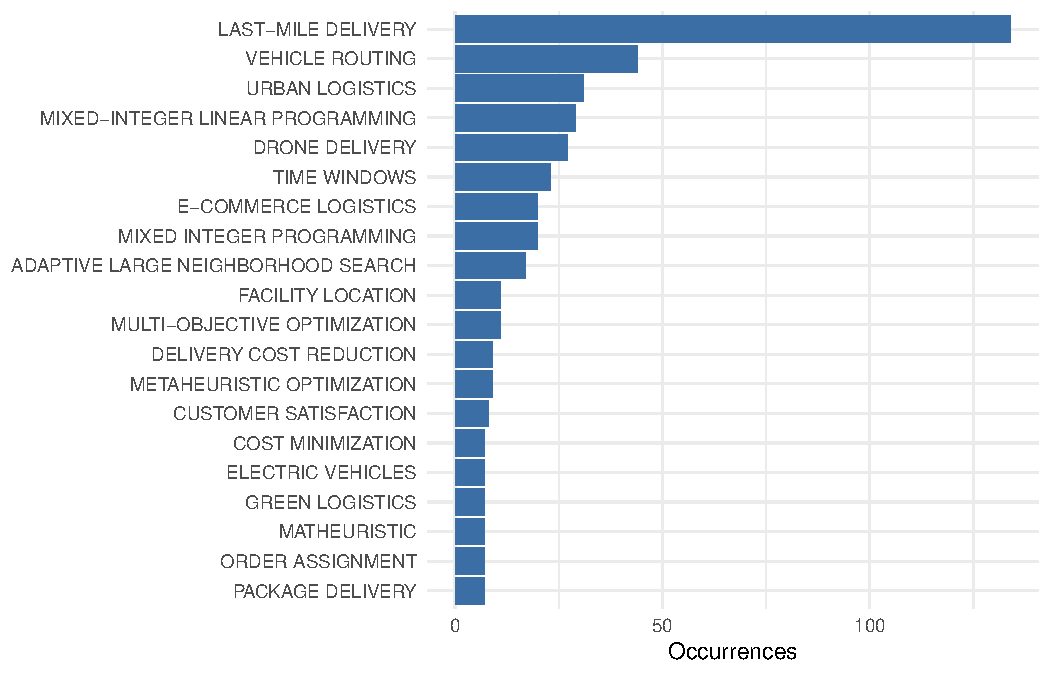
\includegraphics[width=\linewidth]{top_keywords.pdf}
\caption{Most frequent keywords in the \BibIncluded{} included articles (keyword co-occurrence network in the repository: \texttt{biblio/figures/keyword\_cooccurrence.png}).}\label{fig:cooc}
\end{figure}

\begin{figure}[ht]
\centering
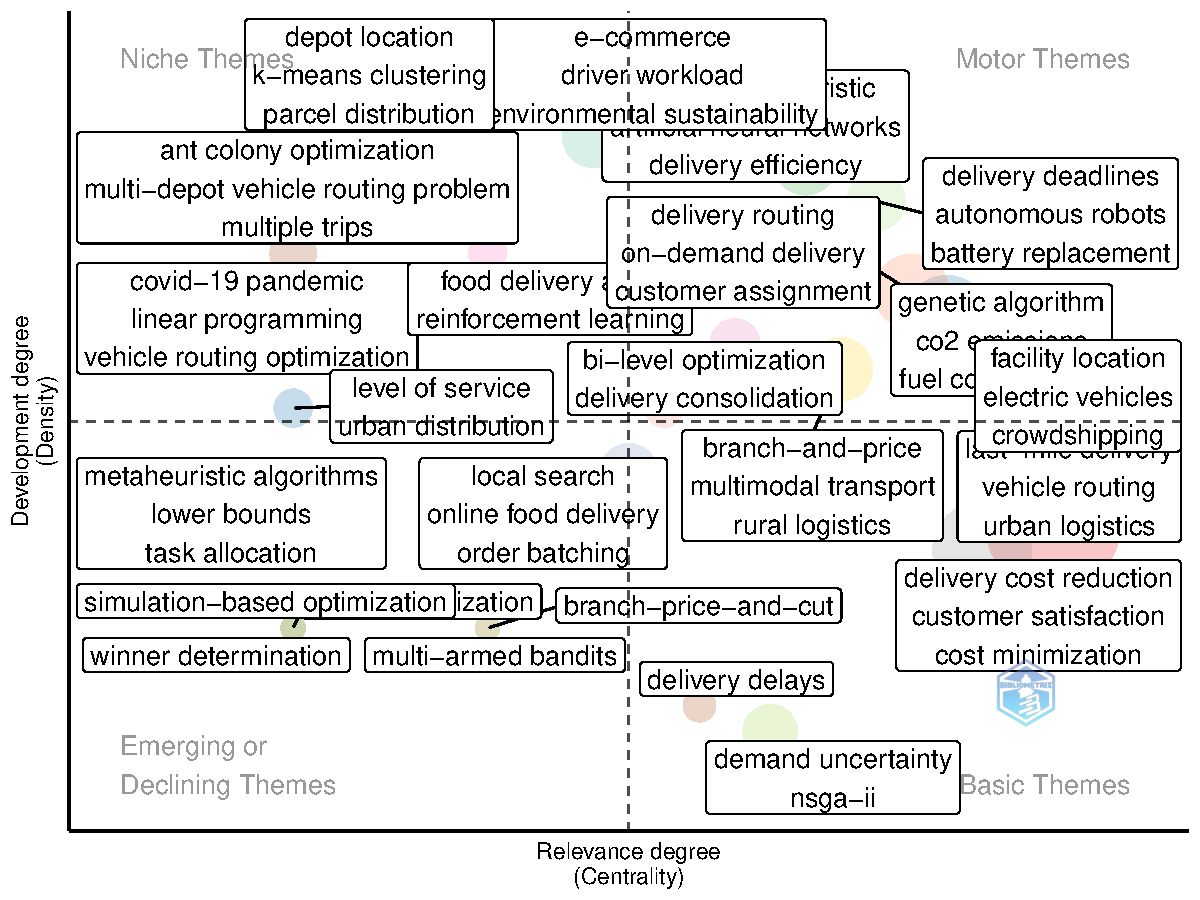
\includegraphics[width=\linewidth]{thematic_map.pdf}
\caption{Thematic map (centrality vs.\ density of keyword clusters).}\label{fig:thematic}
\end{figure}

The intellectual base, measured by co-citation, is anchored in routing. The most co-cited works are the drone-assisted travelling salesman problem of \citet{murray2015} and its successors \citep{agatz2018,sacramento2019}, Solomon's time-window benchmarks \citep{solomon1987}, the adaptive large neighbourhood search of \citet{ropke2006}, the survey of last-mile concepts by \citet{boysen2020}, and two-echelon covering with cargo bikes and lockers \citep{enthoven2020}.

\subsection{Thematic synthesis}

Table~\ref{tab:core} codes 16 core studies selected for citations per year and for proximity to our problem.

\begin{table*}[t]
\centering\scriptsize
\caption{Core studies (coded from abstracts).}\label{tab:core}
% ---- begin generated/tab_core.tex
\begin{tabular}{p{0.18\linewidth}p{0.28\linewidth}p{0.28\linewidth}p{0.12\linewidth}}
\toprule
Study & Problem & Method & Data \\
\midrule
\citet{deutsch2017} & parcel locker network location & 0-1 ILP / uncapacitated facility location & real \\
\citet{zhou2017} & two-echelon VRP with pickup-facility delivery options & hybrid multi-population genetic algorithm & benchmark + real instance \\
\citet{schermer2019} & VRP with drones and en route launch/retrieval & MILP with valid inequalities; VNS/tabu search & synthetic/ benchmark \\
\citet{liu2019} & online drone fleet dispatch for on-demand meal delivery & MIP with rolling-horizon progressive algorithm & simulation \\
\citet{chen2021} & VRPTW with vans carrying delivery robots & ALNS heuristic & synthetic/ benchmark \\
\citet{alfandari2021} & truck routing with autonomous delivery robots (tardiness) & MIP, branch-and-Benders-cut & synthetic/ benchmark \\
\citet{li2021} & review & literature review of two-echelon truck-UAV routing formulations & none/ review \\
\citet{zhang2022} & dynamic VRP with stochastic requests & knapsack-based linear approximations, multi-stage optimization & real \\
\citet{simoni2023} & crowdsourced food delivery order batching and assignment & graph-based heuristic, local search, agent-based simulation & real \\
\citet{mao2025} & meal delivery order dispatch & survival analysis, instrumental variables, simulation-based evaluation & real \\
\citet{shuaibu2025} & review of last-mile optimisation approaches & literature review & none/ review \\
\citet{zamal2025} & stochastic dynamic order assignment and two-echelon dispatching & MDP, cost function approximation + ALNS & real \\
\citet{voigt2025} & dynamic stochastic some-day delivery (multi-period PCVRPTW) & hybrid ALNS & synthetic/ benchmark \\
\citet{bhattacharya2026} & quick-commerce order allocation balancing fairness and efficiency & minimum-cost assignment, two-stage heuristic & real \\
\citet{luo2026} & micro-fulfillment center location-allocation for instant retailing & integer programming, branch-and-bound with Lagrangian relaxation & real \\
\citet{carlsson2026} & delivery zoning & VRP-based Voronoi partitioning, subgradient algorithm & real \\
\bottomrule
\end{tabular}
% ---- end generated/tab_core.tex

\end{table*}

\paragraph{Vehicle routing with new delivery modes.} The largest stream extends the vehicle routing problem to two-echelon systems, delivery options and new vehicles: multi-depot two-echelon routing with delivery options \citep{zhou2017}, trucks with drones \citep{schermer2019,liu2019}, and trucks launching delivery robots solved by adaptive large neighbourhood search \citep{chen2021} or Benders decomposition \citep{alfandari2021}. Reviews classify these truck--drone formulations \citep{li2021} and summarise the broader toolbox of exact, metaheuristic and learning-based approaches \citep{shuaibu2025}. The stream is methodologically rich but mostly tested on synthetic benchmarks.

\paragraph{On-demand and dynamic delivery.} A second stream treats orders that arrive in real time: batching and assignment for crowdsourced food delivery \citep{simoni2023}, large-scale dynamic routing with stochastic requests \citep{zhang2022}, end-to-end order assignment and dispatch formulated as a Markov decision process \citep{zamal2025}, and dispatch policies evaluated on platform data, where maximising future orders outperforms minimising delay \citep{mao2025}. Delivery time is usually a performance measure here. \citet{voigt2025} are a notable exception: offering a ``some-day'' option yields large cost savings for small increases in delivery time---the closest analogue in the corpus to pricing a delivery promise.

\paragraph{Location of fulfilment infrastructure.} Location models appear in \BibLocation{} studies, from parcel-locker networks reduced to uncapacitated facility location \citep{deutsch2017} to micro-fulfilment location--allocation for instant retail \citep{luo2026}, building on covering models \citep{toregas1971,church1974}. Outside the screened corpus, \citet{kewalramani2023} site Indian dark stores heuristically under delivery-radius constraints.

\paragraph{Fairness and the workforce.} Only \BibWelfare{} studies consider couriers' or drivers' welfare. \citet{bhattacharya2026} show for quick-commerce order allocation that a fairness weight raises delivery time by 4--5\% but cuts earnings inequality by a third, and \citet{carlsson2026} design equitable delivery zones that cut the maximum work span by about a fifth in a field implementation. Neither treats rider \emph{speed} or safety as a constraint.

\subsection{Research gaps}

The bibliometric evidence supports three gaps. First, quick commerce is almost absent: only \BibQComm{} of \BibIncluded{} articles mention quick commerce, dark stores or micro-fulfilment, and none (\BibIndia) studies India, the largest q-commerce market. Second, the delivery promise is treated as given: only \BibPromise{} articles treat delivery time or speed as something to be chosen or priced. Third, rider welfare is marginal (\BibWelfare{} articles), and none models a safe-speed limit. Our study addresses all three by pricing the promise for an Indian city under an explicit rider-speed constraint.
% ---- end sections/literature

% ---- begin sections/methodology
\section{Research methodology}\label{sec:method}

\subsection{Bibliometric data collection}

The course protocol prescribes an EBSCOhost search with the mandatory terms ``operations'' AND ``research''. Because EBSCO requires an institutional login, we ran the identical protocol on OpenAlex, an open index of scholarly works with abstracts, keywords, citation counts and reference lists, on \BibSearchDate. The Boolean string was
\begin{quote}\footnotesize\ttfamily\raggedright
"operations" AND "research" AND ("last-mile" OR "last mile" OR "on-demand delivery" OR "instant delivery" OR "quick commerce" OR "q-commerce" OR "meal delivery" OR "dark store" OR "micro-fulfil*" OR "crowdshipping") AND ("facility location" OR "covering" OR "assignment" OR "vehicle routing" OR "integer programming" OR "linear programming")
\end{quote}
restricted to journal articles in English published 2015--2026. OpenAlex throttles long Boolean queries, so each topic term was queried separately on titles and abstracts and the union (\BibIdentified{} records) was filtered locally: the method clause on title and abstract (\BibAfterMethod{} records) and the mandatory terms on title, abstract, journal name and keywords---approximating EBSCO's default search fields---leaving \BibScreened{} records with no duplicates (Figure~\ref{fig:prisma}).

Titles and abstracts were screened against explicit criteria: a record was included if its primary contribution concerned the last-mile delivery of goods, food or parcels to end customers \emph{and} it developed, applied or reviewed an OR method. Excluded records were coded as out of scope (\BibExclScope; e.g.\ ``last mile'' in disaster relief, health access or passenger transit), without an OR method (\BibExclNoOR; e.g.\ adoption surveys) or editorial (\BibExclIntro). Screening was run in two passes: a first pass screened all records and flagged 24 as uncertain, and an independent second pass re-screened the flagged records, whose decision was adopted (it excluded nine of them, mostly generic routing studies without a last-mile focus). Every decision, its code and the second-pass rationale are recorded in the screening log. \BibIncluded{} articles were retained. Records and cited references were converted to the Bibliometrix format \citep{aria2017bibliometrix} for performance analysis and science mapping; citation counts are OpenAlex counts. Included records were exported to RIS for the Mendeley library.

\begin{figure}[ht]
\centering
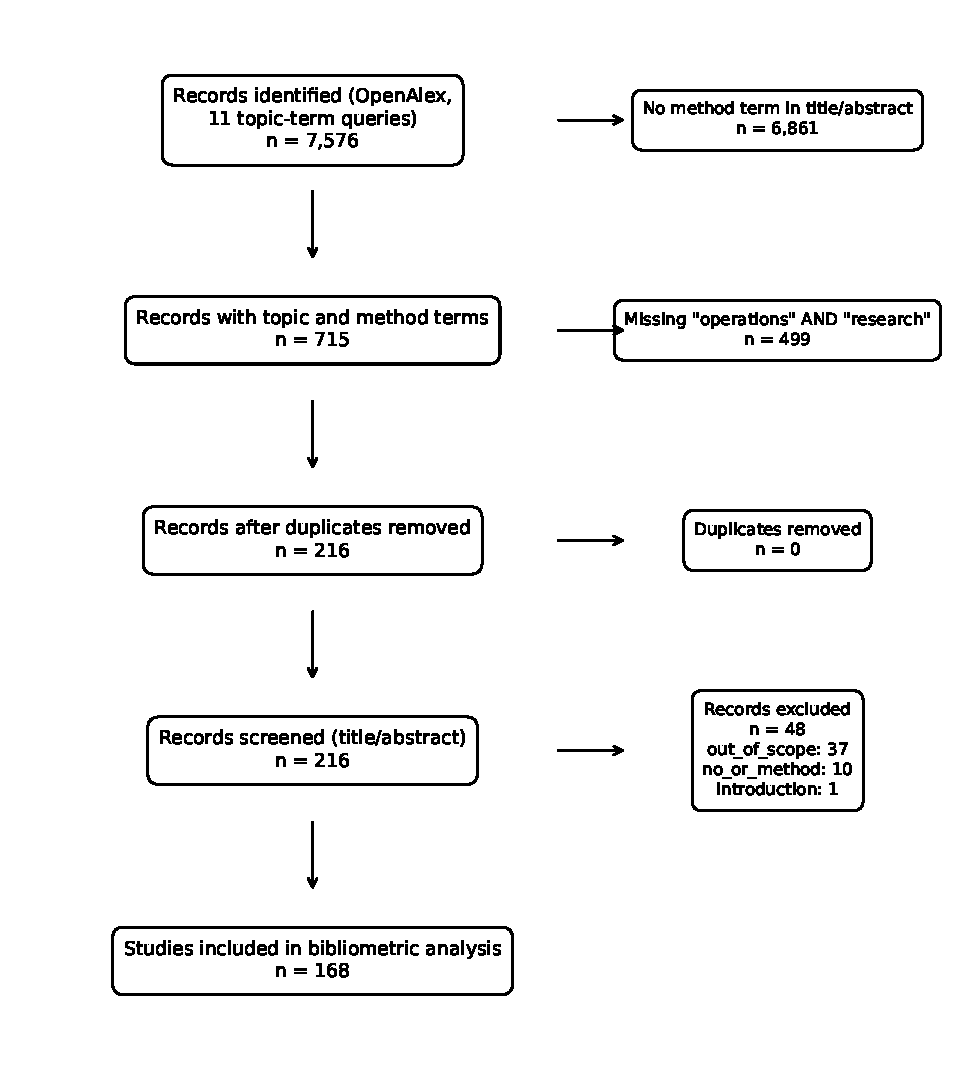
\includegraphics[width=\linewidth]{prisma_flow.pdf}
\caption{Identification and screening of records.}\label{fig:prisma}
\end{figure}

\subsection{Modelling framework}

The case study links four classical OR models at three planning levels (Figure~\ref{fig:chain}). Strategically, a coverage-constrained facility-location model (M1) opens dark stores and allocates demand so that every served household is reachable within the promise $T$ at a safe rider speed $v$, at minimum store and rider cost; rider requirements follow from cycle times (M2). Tactically, a transportation model (M3) plans daily replenishment from mother hubs to the chosen stores. Operationally, an assignment model (M4) dispatches riders to orders in a peak batch, and a PERT model (M5) converts the variability of picking, dispatch and riding into the probability that an order meets $T$. The promise $T$ and speed $v$ are swept as policy parameters; everything else is calibrated from public sources (Section~\ref{sec:data}).

\begin{figure*}[t]
\centering
\begin{adjustbox}{max width=\linewidth}
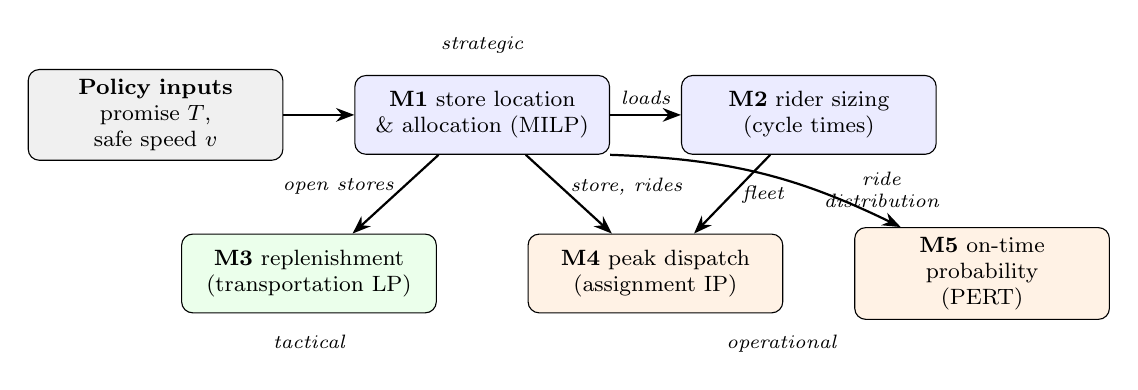
\begin{tikzpicture}[
  box/.style={draw, rounded corners, align=center, font=\footnotesize, minimum height=1.0cm, text width=3.0cm, fill=#1},
  box/.default=white, arr/.style={-{Stealth}, thick}, lab/.style={font=\scriptsize\itshape, align=center}]
  \node[box=gray!12] (pol) {\textbf{Policy inputs}\\ promise $T$, safe speed $v$};
  \node[box=blue!8, right=0.9cm of pol] (m1) {\textbf{M1} store location\\ \& allocation (MILP)};
  \node[box=blue!8, right=0.9cm of m1] (m2) {\textbf{M2} rider sizing\\ (cycle times)};
  \node[box=green!8, below=1.0cm of m1, xshift=-2.2cm] (m3) {\textbf{M3} replenishment\\ (transportation LP)};
  \node[box=orange!10, below=1.0cm of m1, xshift=2.2cm] (m4) {\textbf{M4} peak dispatch\\ (assignment IP)};
  \node[box=orange!10, right=0.9cm of m4] (m5) {\textbf{M5} on-time probability\\ (PERT)};
  \draw[arr] (pol) -- (m1);
  \draw[arr] (m1) -- node[lab, above] {loads} (m2);
  \draw[arr] (m1) -- node[lab, left, pos=0.4] {open stores} (m3);
  \draw[arr] (m1) -- node[lab, right, pos=0.4] {store, rides} (m4);
  \draw[arr] (m2) -- node[lab, right] {fleet} (m4);
  \draw[arr] (m1.south east) to[bend left=12] node[lab, right, pos=0.7] {ride\\ distribution} (m5);
  \node[lab, above=0.15cm of m1] {strategic};
  \node[lab, below=0.15cm of m3] {tactical};
  \node[lab, below=0.15cm of m4, xshift=1.6cm] {operational};
\end{tikzpicture}
\end{adjustbox}
\caption{Model chain linking strategic, tactical and operational decisions.}
\label{fig:chain}
\end{figure*}

All models are implemented in Python with PuLP and solved with HiGHS; code, data provenance and a test suite verifying each model against hand-solvable or brute-force instances accompany the paper as supplementary material.
% ---- end sections/methodology

% ---- begin src/ai_statement.tex
\subsection{Use of generative AI}\label{sec:ai}

As required by Springer Nature policy, we note that a large language model (Claude, Anthropic) was used for language polishing of the manuscript text and for assistance with code development and document formatting. The study design, literature screening, modelling, analysis and interpretation were carried out by the authors. The authors reviewed and edited all AI-assisted output and take full responsibility for the content of the article.
% ---- end src/ai_statement.tex

% ---- begin sections/data
\section{Case and data}\label{sec:data}

\subsection{Study area}

The study area is the Bruhat Bengaluru Mahanagara Palike (BBMP) as delimited into 243 wards in 2022 \citep{opencity2022wards}; the ward polygons cover \AreaKm~km\textsuperscript{2}, consistent with the official 712.5~km\textsuperscript{2}. Bengaluru hosts roughly \CurrentStores{} dark stores of the three largest platforms \citep{qcmap2026}, making it the most contested q-commerce market in India.

\subsection{Data sources and audit}

Table~\ref{tab:sources} lists the inputs. Demand is spatialised with the WorldPop 2025 constrained population grid at 100~m \citep{worldpop2025}, aggregated to \NDemandCells{} cells of about 0.46~km. WorldPop sums to \PopWorldPop~million inside BBMP---below the 2011 Census count of 8.44 million \citep{census2011}---because it caps density in the dense core; we therefore keep its spatial pattern and scale it to the census total. Candidate store sites are the \NOsmSites{} supermarkets, grocery and convenience shops and warehouses mapped in OpenStreetMap within BBMP \citep{osm2026}, merged into \NCandidates{} candidate locations. Road distances are straight-line distances multiplied by a detour factor of \Detour{} (interquartile range \DetourLo--\DetourHi), the median road/straight-line ratio over a random sample of OSRM routes.

\begin{table*}[t]
\centering\small
\caption{Data sources.}\label{tab:sources}
\begin{tabular}{p{0.20\linewidth}p{0.40\linewidth}p{0.28\linewidth}}
\toprule
Input & Source & Use \\
\midrule
Population & WorldPop R2025A, India 2025, 100~m constrained & Spatial demand weights \\
Boundary & BBMP ward map 2022 (OpenCity) & Study area \\
Candidate sites & OpenStreetMap, Geofabrik extract 2026-10-05 & Possible dark stores \\
Road detour & OSRM, OSM road network & Distance correction \\
Orders, stores, costs & Eternal and Swiggy shareholder letters Q1~FY27; press & Calibration (Table~\ref{tab:params}) \\
\bottomrule
\end{tabular}
\end{table*}

Two popular Kaggle datasets on Indian food and grocery delivery were evaluated and rejected. In the food-delivery dataset, \KaggleOffsetPct\% of delivery points equal the restaurant coordinates plus an identical latitude--longitude offset drawn from 13 values, and road-traffic level is fully determined by the hour of day; the delivery geometry and timing are synthetic. The Blinkit sales dataset uses placeholder e-mail domains for all customers. Neither can support distance-based modelling, a caution for the many studies that use them.

\subsection{Parameters}

Table~\ref{tab:params} summarises the calibration. Bengaluru demand is estimated as stores per platform times orders per store per day: Blinkit \citep[derived from net order value per store per day and average order value]{eternal2026q1}, Swiggy Instamart \citep[1,089 orders per store per day]{swiggy2026q1} and Zepto (mean of the two), giving about 600,000 orders per day. Rider cost uses the average of INR~102 per logged-in hour reported by Eternal for 2025 \citep{goyal2026earnings}. Speeds and pick-pack times follow statements by platform founders \citep{palicha2022,dhindsa2021}. As a validation, the implied rider cost per order in the base case falls within the reported per-order pay of INR~25--35.

\begin{table*}[t]
\centering\small
\caption{Model parameters (base value and sensitivity range).}\label{tab:params}
\begin{tabular}{p{0.28\linewidth}p{0.22\linewidth}p{0.38\linewidth}}
\toprule
Parameter & Base (range) & Basis \\
\midrule
Delivery promise $T$ & 10, 15, 20, 30 min & Policy scenarios \\
Safe rider speed $v$ & 15 (12--20) km/h & \citet{palicha2022} \\
Pick + pack (PERT $a,m,b$) & 1.3, 2, 4 min & \citet{dhindsa2021}; Zepto 76~s \\
Rider assignment; handover & (0, 0.5, 2); (0.5, 1, 2) min & Assumption \\
Daily orders, Bengaluru & 600k (450k--750k) & \citet{eternal2026q1,swiggy2026q1,qcmap2026} \\
Peak-hour share of daily orders & 0.10 (0.08--0.12) & Assumption (evening peak) \\
Store fixed cost & INR 8 (6--11) lakh/month & Opex + capex/60 months \\
Rider cost & INR 125 (102--154)/h & \citet{goyal2026earnings} \\
Rider utilisation & 0.6 (0.5--0.7) & Assumption \\
\bottomrule
\end{tabular}
\end{table*}
% ---- end sections/data

% ---- begin sections/model
\section{Model formulation}\label{sec:model}

\paragraph{Notation.} $I$ is the set of demand cells with daily orders $q_i$ and peak-hour orders $\lambda_i = s\,q_i$ (peak share $s$); $J$ is the set of candidate sites; $d_{ij}$ is road distance. Fulfilment comprises pick-and-pack, rider assignment and handover with PERT means $t^{pp}, t^{as}, t^{ho}$, so the ride radius available under promise $T$ (min) and safe speed $v$ (km/h) is
\begin{equation}
r(T,v) = \frac{v}{60}\left(T - t^{pp} - t^{as} - t^{ho}\right).
\end{equation}
The reachable arcs are $A = \{(i,j): d_{ij} \le r(T,v)\}$.

\paragraph{M1: coverage-constrained network design.} With binary $y_j$ (open site $j$), continuous $x_{ij}$ (share of cell $i$ served by $j$) and $u_i$ (unreachable demand),
\begin{align}
\min\quad & F \sum_{j\in J} y_j + \sum_{(i,j)\in A} c_{ij}\,x_{ij} + M\sum_{i\in I} u_i \label{eq:obj}\\
\text{s.t.}\quad & \sum_{j:(i,j)\in A} x_{ij} + u_i = 1 && \forall i\in I \label{eq:serve}\\
& x_{ij} \le y_j && \forall (i,j)\in A \label{eq:link}\\
& x_{ij}\ge 0,\; u_i \ge 0,\; y_j\in\{0,1\}, \notag
\end{align}
where $F$ is the monthly fixed cost of a store and
\begin{equation}
c_{ij} = 30\, q_i \left(\frac{2 d_{ij}}{v} + \frac{t^{ho}}{60}\right)\frac{w}{\rho}
\end{equation}
is the monthly rider cost of serving cell $i$ from $j$: a round trip at the safe speed plus handover, paid at $w$ per logged-in hour with utilisation $\rho$. The promise enters as a hard restriction on $A$. Cells with no reachable candidate are served by $u_i$ at a large penalty $M$ and reported as unreachable rather than making the model infeasible. Without capacity limits $x_{ij}$ is integral at the optimum, so M1 is an uncapacitated facility-location problem on the reachable arcs; for $T=10$ it reduces to a set-covering structure \citep{toregas1971}, while for loose promises the cost trade-off dominates.

\paragraph{M2: rider sizing.} Each cell is served by its assigned store; peak riders at store $j$ follow from cycle times (Little's law),
$R_j = \big\lceil \sum_{i:\,j(i)=j} \lambda_i \,(2 d_{ij}/v + t^{ho}/60) \big\rceil$.

\paragraph{M3: replenishment (transportation problem).} Open stores are restocked daily from three mother hubs located at OpenStreetMap warehouse sites nearest the demand-weighted centroids of the store network. With hub supplies $a_h$, store requirements $b_j$ and distances $d_{hj}$,
$\min \sum_{h,j} d_{hj} z_{hj}$ subject to $\sum_j z_{hj} = a_h$, $\sum_h z_{hj} = b_j$, $z\ge 0$. We compare the optimum with Vogel's approximation and the north-west corner rule.

\paragraph{M4: peak dispatch (assignment problem).} At a representative store we simulate a 10-minute peak batch of orders with arrival times $\alpha_o$, ready times $\alpha_o + t^{pp} + t^{as}$ and ride times $\tau_o$, and rider \emph{slots} $k$ (a rider's successive trips) that become free at $\phi_k$. The lateness of serving order $o$ with slot $k$ is $\ell_{ko} = \max\{0,\ \max(\phi_k, \alpha_o + t^{pp} + t^{as}) + \tau_o + t^{ho} - (\alpha_o + T)\}$. The assignment model $\min \sum_{k,o} \ell_{ko} x_{ko}$ with $\sum_k x_{ko}=1$, $\sum_o x_{ko}\le 1$, $x\in\{0,1\}$ is compared with first-in-first-out dispatch.

\paragraph{M5: fulfilment reliability (PERT).} An order passes four sequential activities: pick-and-pack, rider assignment, ride and handover. The first, second and fourth use the three-point estimates in Table~\ref{tab:params}; the ride uses the 5th, 50th and 95th percentiles of demand-weighted ride times in the designed network. With PERT means $\mu_k = (a_k + 4m_k + b_k)/6$ and variances $\sigma^2_k = ((b_k-a_k)/6)^2$, the probability of fulfilment within $T$ is $\Phi\big((T-\sum_k\mu_k)/\sqrt{\sum_k \sigma_k^2}\big)$ \citep{malcolm1959}. We also report the rider speed needed to reach 95\% on-time delivery for a given network.
% ---- end sections/model

% ---- begin sections/results
\section{Results}\label{sec:results}

\subsection{Network design across promises and speeds}

Table~\ref{tab:e1} and Figure~\ref{fig:price} report the cost-minimising networks (M1--M2) for every combination of promise $T$ and safe speed $v$. Of the \NMilps{} mixed-integer programs solved for this paper, \NMilpsOptimal{} were proven optimal within HiGHS's default gap tolerance (the longest took \MaxSolveS~s); the remaining \NMilpsLimit{}---maximal covering with 50 and 100 stores at $T=15$ (Section~\ref{sec:frag})---stopped at the 600-second limit, so their reported coverage is a lower bound. Three results stand out.

\begin{table*}[t]
\centering\small
\caption{Cost-minimising dark-store networks for Bengaluru (M1--M2). Cost per order is per \emph{served} order and includes store and rider costs.}\label{tab:e1}
% ---- begin generated/tab_e1.tex
\begin{tabular}{rrrrrrrr}
\toprule
$T$ & $v$ & Radius & Stores & Reachable & Riders & Orders/ & Cost/order \\
(min) & (km/h) & (km) & & pop.\ (\%) & (peak) & store/day & (INR) \\
\midrule
10 & 12 & 1.21 & 390 & 79.3 & 6,705 & 1,220 & 50.4 \\
10 & 15 & 1.51 & 320 & 86.7 & 6,902 & 1,626 & 43.4 \\
10 & 20 & 2.01 & 226 & 94.2 & 6,872 & 2,501 & 35.6 \\
15 & 12 & 2.21 & 270 & 95.9 & 10,295 & 2,130 & 49.3 \\
15 & 15 & 2.76 & 240 & 98.3 & 9,275 & 2,458 & 43.2 \\
15 & 20 & 3.68 & 203 & 99.8 & 7,929 & 2,950 & 36.3 \\
20 & 12 & 3.21 & 261 & 99.4 & 11,341 & 2,286 & 50.8 \\
20 & 15 & 4.01 & 239 & 99.9 & 9,700 & 2,509 & 43.9 \\
20 & 20 & 5.34 & 204 & 100.0 & 7,968 & 2,941 & 36.4 \\
30 & 12 & 5.21 & 260 & 100.0 & 11,553 & 2,308 & 51.2 \\
30 & 15 & 6.51 & 238 & 100.0 & 9,733 & 2,521 & 43.9 \\
30 & 20 & 8.68 & 202 & 100.0 & 7,987 & 2,970 & 36.4 \\
\bottomrule
\end{tabular}
% ---- end generated/tab_e1.tex

\end{table*}

\begin{figure*}[t]
\centering
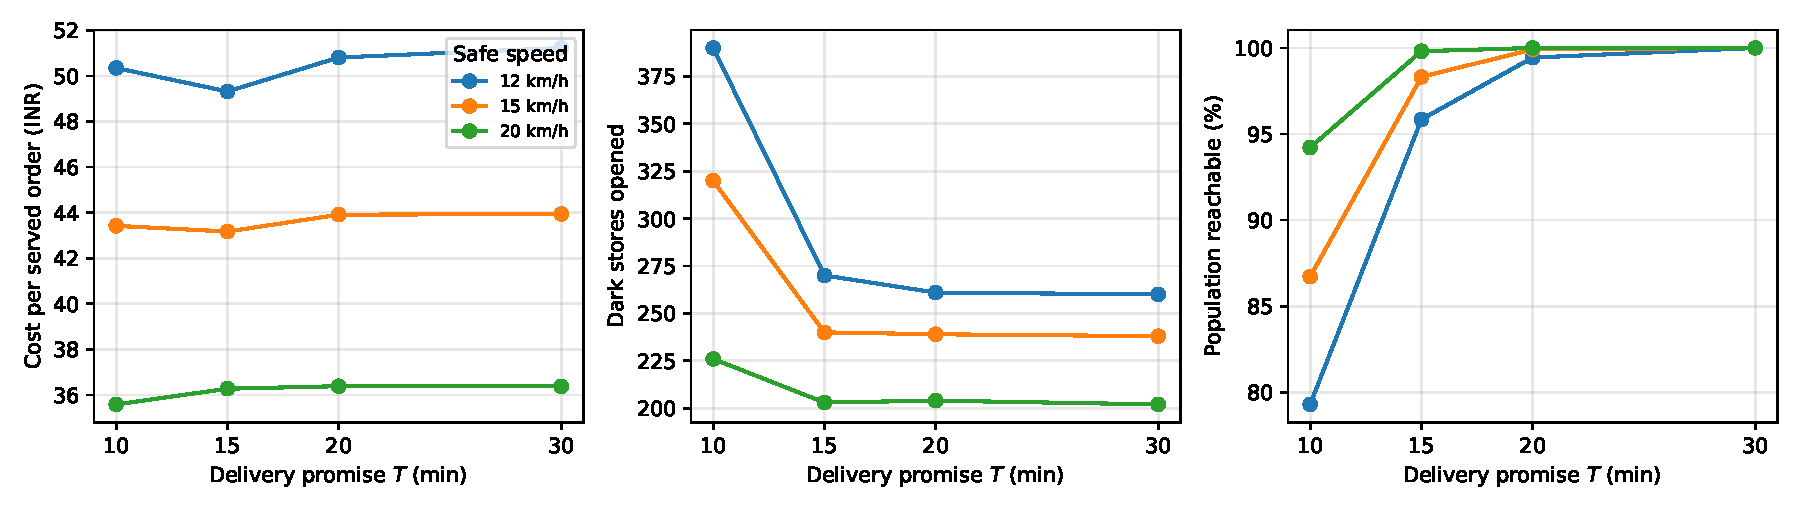
\includegraphics[width=\linewidth]{price_of_speed.pdf}
\caption{The price of speed: cost per served order, stores opened and share of residents reachable, by promise $T$ and safe rider speed $v$.}\label{fig:price}
\end{figure*}

\paragraph{The promise decides \emph{who} is served, not what it costs.} At a safe speed of \BaseV~km/h, a 15-minute promise reaches \ServedFifteenPct\% of residents with \StoresTFifteen{} stores at INR~\CostPerOrderFifteen{} per order. Tightening to 10 minutes raises the store count to \StoresTTen{} but leaves \UnreachTenPct\% of residents---mostly at the city's edge, where retail stock suitable for dark stores is sparse---with no candidate site within reach (Figure~\ref{fig:maps}); the cost per served order barely moves (INR~\CostPerOrderTen{}). Relaxing the promise beyond 15 minutes changes almost nothing: the cost-optimal network has about \StoresTTwenty{} stores whether the promise is 20 or 30 minutes, because the cost trade-off between stores and rider time, not the promise, then determines the radius.

\paragraph{The speed cap decides what it costs.} Because riders are paid per logged-in hour, cost per order falls steeply with rider speed: at $T=15$ it is INR~\CostPerOrderVTwelve{} at 12~km/h, \CostPerOrderFifteen{} at 15~km/h and \CostPerOrderVTwenty{} at 20~km/h. Capping speed at 15 rather than 20~km/h costs about \SpeedCapPremiumPct\% more per order. This is the platform's economic incentive to push speed---independent of the advertised promise---and the quantity a regulator implicitly prices when it sets a speed norm.

\paragraph{The cost-optimal network is smaller than today's.} A single network serving all of Bengaluru's demand at minimum cost needs \StoreRange{} stores across the scenarios, against roughly \CurrentStores{} operated by three competing platforms today. The gap is a measure of the duplication that competition creates.

\begin{figure*}[t]
\centering
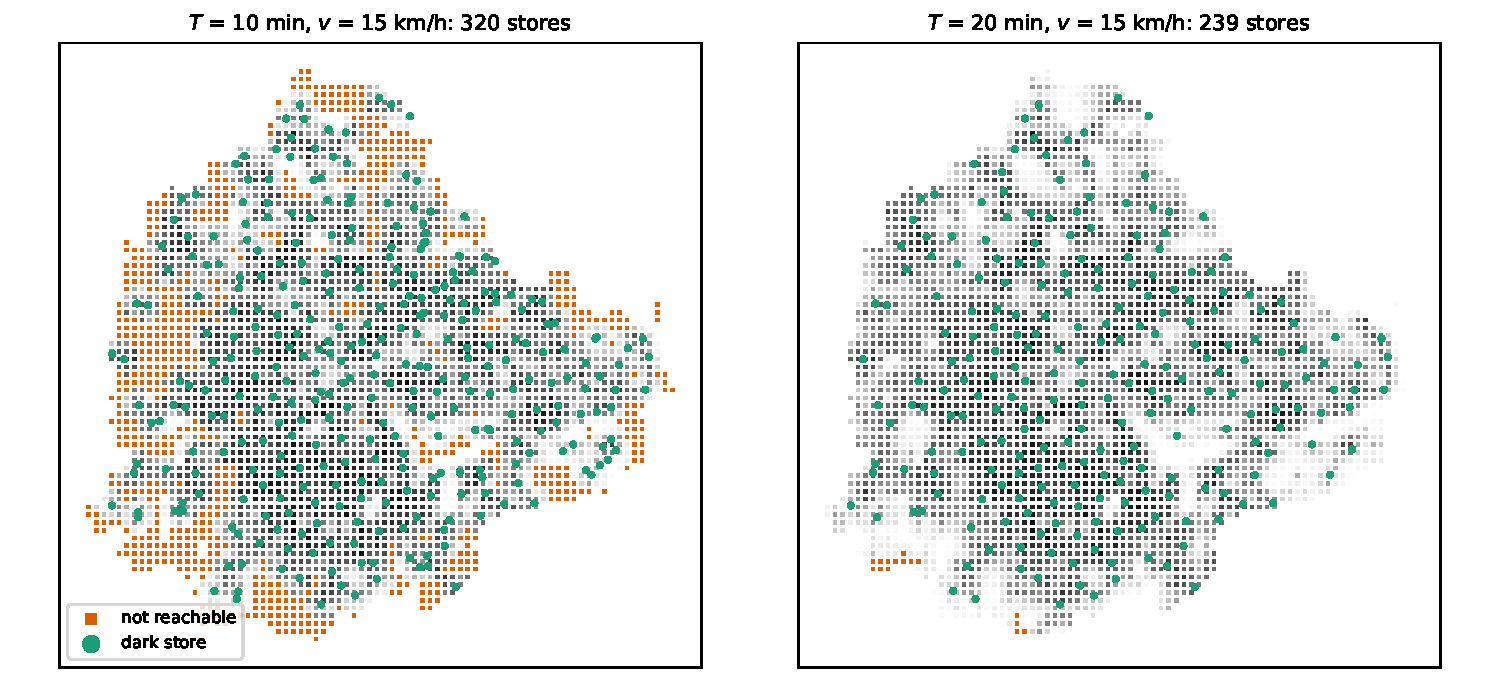
\includegraphics[width=\linewidth]{network_maps.pdf}
\caption{Optimal networks for $T=10$ and $T=20$ minutes at 15~km/h. Grey cells are served; orange cells have no candidate site within reach.}\label{fig:maps}
\end{figure*}

\paragraph{The price of speed at equal coverage.} The coverage gap at $T=10$ arises because mapped retail sites are scarce at the city's edge. Allowing a store anywhere on a $\sim$0.9~km lattice of populated cells (\GridCandidates{} candidate sites), a 10-minute promise reaches \GridTenServedPct\% of residents but needs \GridTenStores{} stores at INR~\GridTenCost{} per order, against \GridFifteenStores{} stores at INR~\GridFifteenCost{} for 15 minutes. Serving \emph{everyone} within 10 rather than 15 minutes therefore needs \GridStorePremiumPct\% more stores and costs \GridCostPremiumPct\% more per order---about INR~\GridPricePerMinute{} per order for each minute saved. The price of the last five minutes is paid mainly in real estate at the periphery, which the platforms' current networks largely avoid.

\subsection{Fragmentation and a ``realistic promise'' policy}\label{sec:frag}

Figure~\ref{fig:frag} solves the maximal covering problem for a given number of stores placed optimally. Within 15 minutes, 100 well-placed stores already reach at least \FragFifteenHundred\% of residents. Within 10 minutes, 165 stores---Blinkit's Bengaluru network---reach at most \FragTenOne\%, and no number of stores at mapped retail sites lifts coverage above \FragTenMax\%. A 10-minute promise is therefore a promise to the dense core only, whichever platform makes it, and three platforms replicating 150-store networks buy little extra coverage.

\begin{figure}[ht]
\centering
\IfFileExists{fragmentation.pdf}{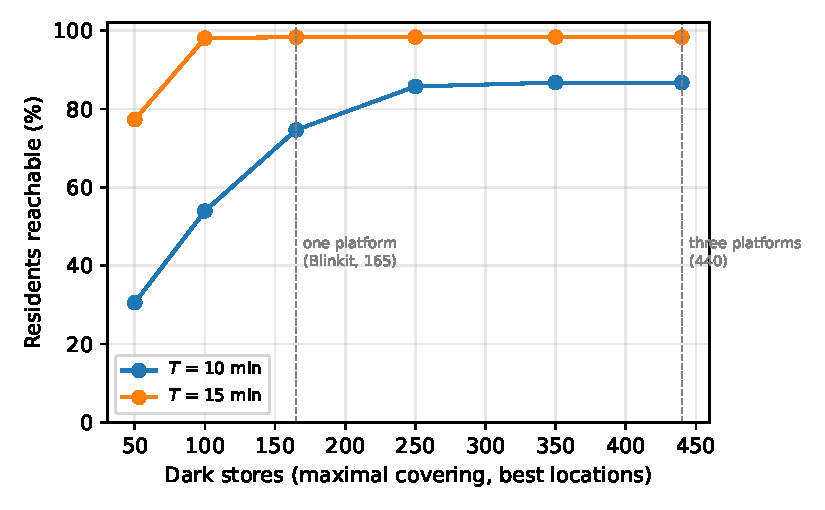
\includegraphics[width=\linewidth]{fragmentation.pdf}}{\todo{fragmentation figure}}
\caption{Share of residents reachable with $P$ optimally located stores (maximal covering, $v=15$~km/h).}\label{fig:frag}
\end{figure}

We also test the operational definition proposed in Section~\ref{sec:discussion}: promise 10 minutes wherever an address lies within the safe 10-minute radius of some candidate site, and 15 minutes elsewhere. This differentiated promise gives \MixedTenShare\% of residents a 10-minute promise and still serves \MixedServed\% overall---the same coverage as a uniform 15-minute promise---with \MixedStores{} stores (\MixedExtraStores{} more) at INR~\MixedCost{} per order, \MixedPremiumPct\% above the uniform 15-minute network. A uniform 10-minute promise, by contrast, reaches only \ServedTenPct\% of residents. Tying the promise to reachability thus delivers 10-minute service to most of the city at a small premium, without leaving anyone unserved and without requiring riders to exceed the safe speed.

\subsection{Fulfilment reliability (PERT)}

Table~\ref{tab:pert} gives the PERT estimate of fulfilment time in each network at 15~km/h. Inside the designed networks every served address is within the ride radius, so on-time probabilities are high: \PertTenP\% at $T=10$. A 10-minute promise met 95\% of the time requires riders to average \PertTenSpeed~km/h in the 10-minute network---below the safe speed. Ten-minute delivery is therefore feasible without speeding, \emph{but only} with a dense network and only for the \ServedTenPct\% of residents that network can reach.

\begin{table}[ht]
\centering\small
\caption{PERT fulfilment time by promise (network designed for that promise, $v=15$~km/h); $v_{95}$ is the rider speed needed for 95\% on-time delivery.}\label{tab:pert}
% ---- begin generated/tab_pert.tex
\begin{tabular}{rrrrr}
\toprule
$T$ & Mean & SD & $P$(on & $v_{95}$ \\
(min) & (min) & (min) & time) & (km/h) \\
\midrule
10 & 7.33 & 0.99 & 0.997 & 12.1 \\
15 & 8.11 & 1.31 & 1.000 & 8.3 \\
20 & 8.23 & 1.40 & 1.000 & 6.0 \\
30 & 8.23 & 1.40 & 1.000 & 5.0 \\
\bottomrule
\end{tabular}
% ---- end generated/tab_pert.tex

\end{table}

\subsection{Peak dispatch (assignment)}

The pressure appears when a network designed for one promise is asked to meet a tighter one. Table~\ref{tab:assign} dispatches a 10-minute peak batch at a stressed store of the 15-minute network (90th percentile of mean ride distance, \AssignStressRide~km). With the full sized fleet, a 15-minute promise is met for every order, but a 10-minute promise only for \AssignStressTenOnTime\%; the late orders could be saved only if riders averaged about \AssignStressSpeed~km/h, above the safe speed. Under lean staffing the gap widens sharply. Optimal assignment reduces total lateness relative to first-in-first-out dispatch, although because it minimises lateness rather than the count of late orders it occasionally delivers fewer orders strictly on time. The pressure is local: at the median-load store, where rides average 0.9~km, 60\% of the sized fleet meets even a 10-minute promise for every order under optimal dispatch (first-in-first-out reaches 90\%), and only at 40\% staffing do orders run late. Tight promises thus fail first at the edges of store catchments, which is where riders would be pushed to speed.

\begin{table*}[t]
\centering\small
\caption{Peak 10-minute batch at a stressed store of the 15-minute network: optimal assignment vs FIFO.}\label{tab:assign}
% ---- begin generated/tab_assign.tex
\begin{tabular}{rrrrrr}
\toprule
Staffing & Riders & $T$ & On time & On time & Mean lateness (min) \\
 & & (min) & optimal & FIFO & optimal / FIFO \\
\midrule
40\% & 32 & 10 & 17\% & 26\% & 4.24 / 4.47 \\
40\% & 32 & 15 & 56\% & 59\% & 0.89 / 1.46 \\
40\% & 32 & 20 & 100\% & 90\% & 0.00 / 0.25 \\
60\% & 47 & 10 & 35\% & 49\% & 1.19 / 1.52 \\
60\% & 47 & 15 & 100\% & 93\% & 0.00 / 0.10 \\
60\% & 47 & 20 & 100\% & 100\% & 0.00 / 0.00 \\
80\% & 63 & 10 & 64\% & 64\% & 0.82 / 0.83 \\
80\% & 63 & 15 & 100\% & 100\% & 0.00 / 0.00 \\
80\% & 63 & 20 & 100\% & 100\% & 0.00 / 0.00 \\
100\% & 79 & 10 & 64\% & 64\% & 0.82 / 0.82 \\
100\% & 79 & 15 & 100\% & 100\% & 0.00 / 0.00 \\
100\% & 79 & 20 & 100\% & 100\% & 0.00 / 0.00 \\
\bottomrule
\end{tabular}
% ---- end generated/tab_assign.tex

\end{table*}

\subsection{Replenishment (transportation)}

For the base network ($T=15$, $v=15$; \StoresTFifteen{} stores), replenishment from three equal-capacity mother hubs costs \TransLP~million order-km per day at the optimum. Vogel's approximation comes within \TransVAMGapPct\% of the optimum, while the north-west corner rule is \TransNWRatio{} times worse. Supplying each store from its nearest hub would cost \TransNearest~million order-km, so equal hub capacities carry a \TransCapPremiumPct\% premium. Because the store count hardly changes beyond 15 minutes, replenishment cost is insensitive to the promise in that range.

\subsection{Sensitivity analysis}

Figure~\ref{fig:tornado} varies each uncertain input over its range at the base case. The cost per order is most sensitive to \TornadoTop{} (a swing of INR~\TornadoTopSpan) and \TornadoSecond{} (INR~\TornadoSecondSpan): rider time dominates the cost structure, which is why speed is the platform's main lever. Higher rider cost or demand raises the optimal number of stores, shortening rides; higher store cost lowers it. Longer pick-and-pack times shrink the ride radius; cost per \emph{served} order changes little because the hardest-to-serve cells drop out, which again shows that tighter time budgets are paid in coverage. The headline findings---a store count near the base case, cost flat in $T$ beyond 15 minutes, and speed as the cost driver---hold across all ranges.

\begin{figure}[ht]
\centering
\IfFileExists{tornado.pdf}{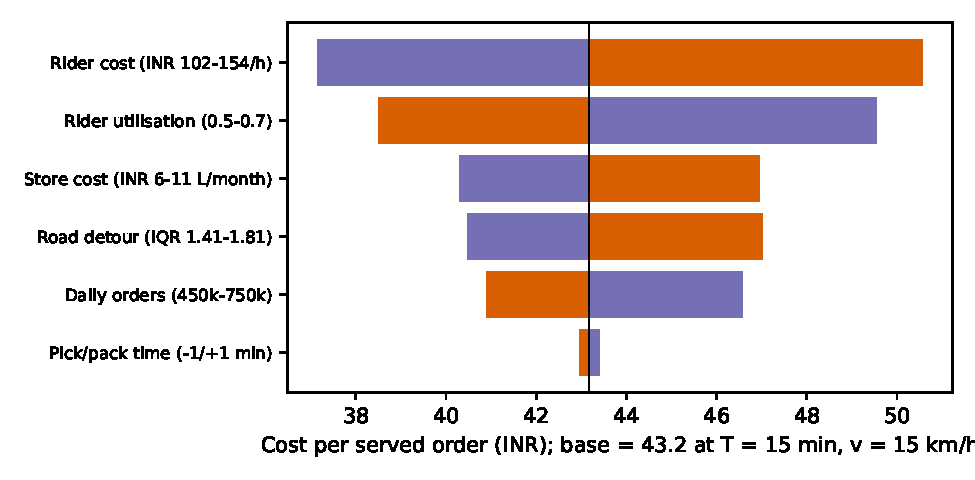
\includegraphics[width=\linewidth]{tornado.pdf}}{\todo{tornado figure pending}}
\caption{One-at-a-time sensitivity of cost per served order ($T=15$, $v=15$).}\label{fig:tornado}
\end{figure}
% ---- end sections/results

% ---- begin sections/discussion
\section{Discussion}\label{sec:discussion}

\subsection{What makes a speed target ``unrealistic''?}

The results separate two quantities that the public debate conflates. The \emph{promise} $T$ is a network-design decision: it determines how many stores are needed and which neighbourhoods can be served. The \emph{speed} riders must sustain is a cost decision: at a given network, faster riding is cheaper for the platform because rider time is paid per hour. A promise becomes unrealistic when the network cannot deliver it at a safe speed. Our results suggest a practical test for regulators: a promise is realistic for an address if the address lies within the safe ride radius of an open store after realistic pick-and-pack time---exactly the reachability set $A$ in M1. By that test, 15 minutes is realistic for \ServedFifteenPct\% of Bengaluru residents with the cost-optimal network, while 10 minutes is realistic for \ServedTenPct\% even with \StoresTTen{} stores. Promising 10 minutes beyond that footprint, or asking a 15-minute network to deliver in 10, can be met only by faster riding (Section~\ref{sec:results}).

\subsection{Managerial implications}

For platforms, the cost per order is nearly flat between 10 and 30 minutes once the network is designed for the promise; the expensive lever is rider speed. Platforms can therefore offer differentiated promises---10 minutes in dense cores, where mapped retail space allows it, and 15 elsewhere---at modest cost (a uniform 10-minute promise for everyone costs about \GridCostPremiumPct\% more per order), and should resist meeting tight promises at peaks through speed. Dispatch quality matters most at stressed stores and lean staffing, where optimal assignment reduces lateness relative to FIFO.

\subsection{Policy implications}

A speed norm is more enforceable than a promise ban. A cap of 15~km/h raises cost per order by about \SpeedCapPremiumPct\% relative to 20~km/h in our base case---a quantifiable price of rider safety that can be weighed against accident risk. Platform disclosures of delivery radius and store density would allow regulators to check reachability directly.

\subsection{Limitations}

Demand is spatialised from residential population and calibrated from platform-level disclosures rather than order data; store counts come from a third-party tracker; candidate sites depend on OpenStreetMap completeness; road distances use a single detour factor and free-flow routing; rider cost is a per-hour average; and the model represents one network rather than three competing platforms. PERT assumes independent activities and a normal approximation. On the bibliometric side, the search used OpenAlex rather than the prescribed EBSCO database, citation counts are OpenAlex rather than Google Scholar counts, and country metadata were too sparse for a reliable country analysis.

\subsection{Future research agenda}

Each gap in Section~\ref{sec:lit} suggests an agenda. For quick commerce: competitive location models in which several platforms site stores in the same city, with capacity and inventory at dark stores. For promises as decisions: models that set differentiated promises jointly with network design, extending the some-day options of \citet{voigt2025} to minutes-scale delivery. For rider welfare: explicit accident-risk functions of speed in the objective, time-dependent travel times, and dynamic dispatch with fairness constraints building on \citet{bhattacharya2026} and \citet{carlsson2026}. For India: validation against platform order data, which would also remove our reliance on population as a demand proxy.
% ---- end sections/discussion

% ---- begin sections/conclusion
\section{Conclusion}\label{sec:conclusion}

\textbf{RQ1.} OR research on last-mile delivery has grown by \BibGrowthPct\% a year since 2015, led by vehicle routing with drones, robots and two-echelon systems solved by mixed-integer programming and large neighbourhood search; quick commerce (\BibQComm{} of \BibIncluded{} articles), India (none) and rider welfare (\BibWelfare) remain almost unstudied, and the delivery promise is rarely a decision variable.
\textbf{RQ2.} In Bengaluru the cost-optimal network has about \StoresTFifteen{} dark stores for any promise of 15 minutes or more; a 10-minute promise cannot reach \UnreachTenPct\% of residents from mapped retail sites, and serving everyone within 10 minutes needs \GridStorePremiumPct\% more stores at \GridCostPremiumPct\% higher cost per order. Rider speed, not the promise, drives cost: a 15~km/h cap costs about \SpeedCapPremiumPct\% more per order than 20~km/h.
\textbf{RQ3.} A promise is realistic where an address lies within the safe ride radius of a store; on that basis 15 minutes is realistic for nearly all of Bengaluru and 10 minutes for \MixedTenShare\% of residents, and a promise differentiated this way costs only \MixedPremiumPct\% more per order than a uniform 15-minute network. Regulating speed norms and disclosure of delivery radii is more meaningful than regulating advertised minutes.
% ---- end sections/conclusion


% ---- begin src/declarations.tex
\bmhead{Acknowledgements}
We thank Dr Vishal Pradhan, instructor of the Operations Research Management course at NMIMS University, Mumbai, for guidance throughout this project, including on the bibliometric research process. We also acknowledge the open data and software on which this study relies: map data \copyright{} OpenStreetMap contributors (ODbL~1.0), obtained via Geofabrik; WorldPop, University of Southampton, for gridded population estimates; OpenCity.in and Devdatta Tengshe for the BBMP ward boundaries; OpenAlex for bibliographic metadata; and the developers of OSRM, PuLP, HiGHS and Bibliometrix.

\section*{Declarations}

\begin{itemize}
\item \textbf{Funding:} No funding was received to assist with the preparation of this manuscript.
\item \textbf{Competing interests:} The authors have no relevant financial or non-financial interests to disclose.
\item \textbf{Ethics approval and consent to participate:} Not applicable. The study uses only publicly available secondary data and involves no human participants.
\item \textbf{Consent for publication:} Not applicable.
\item \textbf{Data availability:} All inputs are public: WorldPop 2025 population (CC BY 4.0), BBMP ward boundaries (OpenCity), OpenStreetMap (ODbL 1.0), OpenAlex bibliographic metadata (CC0) and the cited company disclosures. Processed data, the screening log, provenance records and hashes are available at \RepoURL.
\item \textbf{Materials availability:} Not applicable.
\item \textbf{Code availability:} All code (data acquisition, models, experiments and manuscript generation) is available at \RepoURL{} under the MIT licence.
\item \textbf{Author contributions:} All authors contributed to the study conception and design. Data collection, screening, modelling and analysis were performed by all authors. All authors contributed to drafting and revising the manuscript. All authors read and approved the final manuscript.
\item \textbf{Use of generative AI:} A large language model was used for language polishing and for assistance with code and formatting; see Section~\ref{sec:ai}.
\end{itemize}
% ---- end src/declarations.tex


\bibliography{references}

\end{document}
